\documentclass[tikz,border=2mm]{standalone}
\usetikzlibrary{shapes.geometric}
\begin{document}
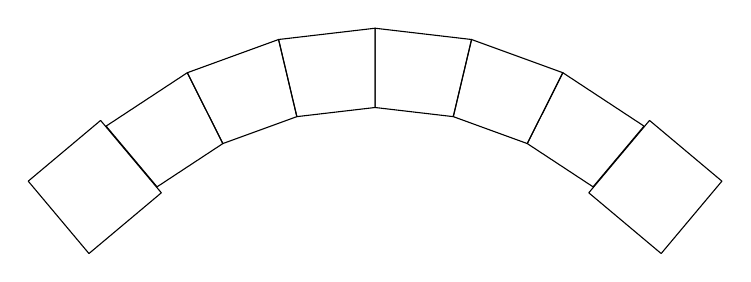
\begin{tikzpicture}[declare function={alpha=40;% opening angle of the bridge 
    n=6;% number of inner bricks
    w=1;% brick height
    beta=alpha/n;% auxiliary angle
},line join=round]
 \pgfmathtruncatemacro{\myn}{n}   
 \path coordinate (tmp) node[anchor=south east,shift={(alpha-90:w*0.1cm)},minimum size=w*1.2cm,rectangle,draw,rotate=alpha](L){}
 foreach \i in {1,...,\myn}
 {node[trapezium,draw,outer sep=0pt,trapezium angle={-90+beta},minimum height=1cm,anchor=bottom left corner,rotate={alpha-2*(\i-0.5)*beta}](t-\i) {}
 (t-\i.bottom right corner) }
 node[anchor=south west,shift={(-alpha-90:w*0.1cm)},minimum size=w*1.2cm,rectangle,draw,rotate=-alpha](R){};   
\end{tikzpicture}    
\end{document}